\item Sea $S=\{(x,y,z):x-y+z=0\}$.
    \begin{enumerate}
        \item Probar que $S$ es un subespacio de $\R^3$ y hallar una base para $S$.
            \begin{mdframed}[style=s]
                \begin{enumerate}
                    \item El vector $(0,0,0)\in S$ ya que $0-0+0=0$
                    \item Sean $s_1=(x_1,y_1,z_1),s_2=(x_2,y_2,z_2)\in S$\\
                        $\to s_1+s_2=(x_1,y_1,z_1)+(x_2,y_2,z_2)=(x_1+x_2,y_1+y_2,z_1+z_2)$\\
                        De donde, $x_1+x_2-(y_1-y_2)+z_1+z_2=x_1-y_1+z_1+x_2-y_2+z_2=0+0=0\to s_1+s_2\in S$
                    \item Sea $\alpha\in\R,s\in S\to \alpha s=\alpha(x,y,z)=(\alpha x, \alpha y,\alpha z)$\\
                        $\to \alpha x -\alpha y+\alpha z=\alpha(x-y+z)=\alpha 0=0\to\alpha s\in S$
                \end{enumerate}
                Por ende, $S$ es subespacio de $\R^3$\\
                Cualquier elemento de $S$ cumple con $x-y+z=0\to$ sea un $s\in S,s=(y-z,y,z)=y(1,1,0)+z(-1,0,1)$. Como un vector arbitrario de $S$ es combinación lineal de $(1,1,0);(-1,0,1)$, los cuales son li, $B=\{(1,1,0);(-1,0,1)\}$ es una base de $S$. En la Figura 6 se observa el plano $x-y+z=0$, y los dos vectores de la base.
                \begin{center}
                    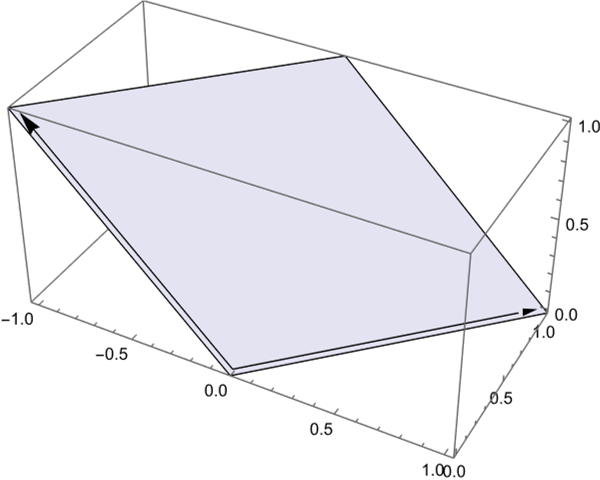
\includegraphics[width=0.4\textwidth]{Ej14.png}\\
                    Figura 6. Plano $x-y+z=0$ con vectores de la base.
                \end{center}
            \end{mdframed}
        \item Hallar un subespacio $T$ de $\R^3$ tal que $S+T=\R^3$¿Es único?
            \begin{mdframed}[style=s]
                Quiero un subespacio que al sumarlo con el plano del inciso anterior obtenga $\R^3$. Lo primero que se me ocurre es en una recta que corte al plano en un único punto y contenga al origen. Al sumar los vectores de esta recta con los del plano me puedo desplazar por todo $\R^3$. Las rectas más sencillas son los ejes coordenados.\\
                En el caso del eje de abscisas, tenemos que $T=\overline{\{(1,0,0)\}}$. Para comprobar que la suma sea realmente $\R^3$ tomemos un vector $v=(x,y,z)$ de $\R^3$. 
                \begin{center}
                    $(x,y,z)=\alpha(1,1,0)+\beta(-1,0,1)+\gamma(1,0,0)$\\
                    $\begin{cases}
                        x=\alpha-\beta+\gamma\\
                        y=\alpha\\
                        z=\beta
                    \end{cases}\to\begin{cases}
                        \gamma=x-y+z
                    \end{cases}$\\
                    $\to v=y(1,1,0)+z(-1,0,1)+(x-y+z)(1,0,0)$
                \end{center}
                Con esto se ve que cualquier vector de $\R^3$ puede ser escrito como la suma de un vector de $S$(en este caso $s=y(1,1,0)+z(-1,0,1)$) y otro de $T$($t=(x-y+z)(1,0,0)$). En la Figura 7 se muestra un caso en particular de esta situación:
                \begin{center}
                    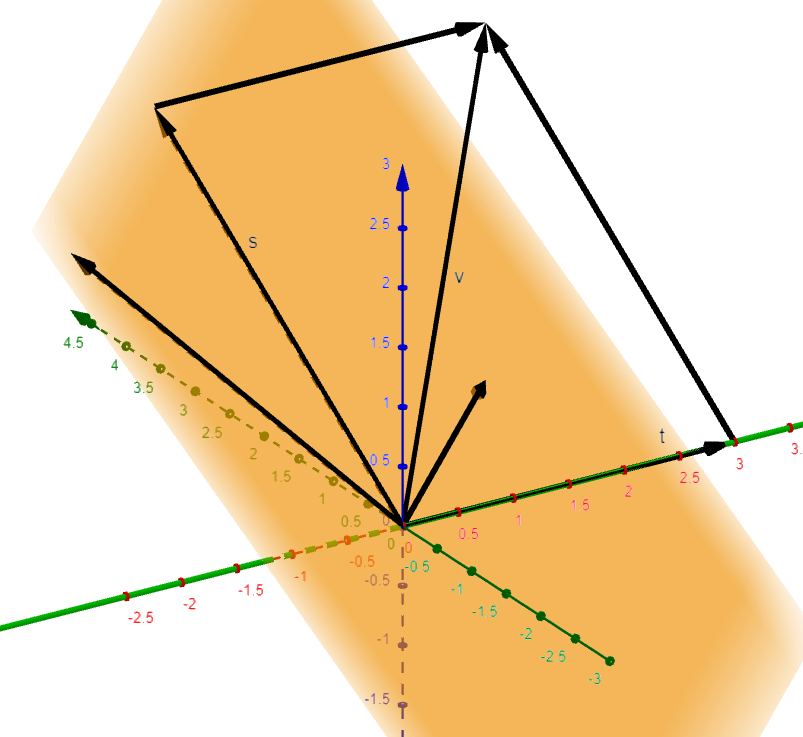
\includegraphics[width=0.4\textwidth]{Ej14b.png}\\
                    Figura 7. $v=(2,2,3)$ como combinación lineal de $s=(2,2,0)+(-3,0,3)$ y $t=(3,0,0)$
                \end{center}
                Un argumento análogo se puede hacer con cualquiera de las rectas mencionadas. ¿Qué sucede con los planos?\\
                Supongamos un plano cualquiera que contenga al origen $\pi:\alpha x+\beta y+\gamma z=0$. Los vectores de dicho plano se pueden escribir como $t=(\frac{-\beta y-\gamma z}{\alpha},y,z)=y(\frac{-\beta}{\alpha},1,0)+z(\frac{-\gamma}{\alpha},0,1)$. Por lo tanto, un elemento $v\in S+T$, siendo $T$ el plano $\pi$ se puede escribir como $v=s+t,\quad s\in S,t\in T$
                \begin{center}
                    $v=(x,y,z)=a(1,1,0)+b(-1,0,1)+c(\frac{-\beta}{\alpha},1,0)+d(\frac{-\gamma}{\alpha},0,1)$\\
                \end{center}
                \begin{itemize}
                    \item Si por ejemplo, $\pi$ fuese el plano $x-y+z=0$, tenemos que $S=T$
                        \begin{center}
                            $\to v=(x,y,z)=a(1,1,0)+b(-1,0,1)+c(1,1,0)+d(-1,0,1)$\\
                            $\to v=(a+c)(1,1,0)+(b+d)(-1,0,1)$
                        \end{center}
                        Osea que los $v$ son generados por dos vectores, entonces $S+T=S$ como era de esperarse.
                    \item En el caso que tenga otro plano $\frac{-\beta}{\alpha}=\lambda\neq 1$.
                        \begin{center}
                            $\to v=(x,y,z)=a(1,1,0)+b(-1,0,1)+c(\lambda,1,0)+d(\epsilon,0,1)$
                        \end{center}
                        Se puede comprobar que $(\epsilon,0,1)=\frac{\epsilon+1}{1-\lambda}(1,1,0)+(-1,0,1)-\frac{\epsilon+1}{1-\lambda}(\lambda,1,0)$
                        \begin{center}
                            $\to v=(x,y,z)=a(1,1,0)+b(-1,0,1)+c(\lambda,1,0)$
                        \end{center}
                        $v$ se escribe como combinación lineal de 3 vectores li (ya que $\lambda\neq -1$), entonces, una base de $S+T$ es $B=\{(1,1,0);(-1,0,1);(\lambda,1,0)\}$. Como la base tiene 3 elementos, $dim(S+T)=3$ y como es subespacio de $\R^3\to S+T=\R^3$.\\
                        También podría haber puesto la condición $\frac{-\beta}{\gamma}=\epsilon\neq -1$ y hubiese llegado a un resultado similar.
                    \item Como último caso, propongo que $T=\R^3$, entonces tendría que un $v\in S+T$ se escribe
                        \begin{center}
                            $v=(x,y,z)=a(1,1,0)+b(-1,0,1)+c(1,0,0)+d(0,1,0)+e(0,0,1)$\\
                            $\to v=c(1,0,0)+d(0,1,0)+e(0,0,1)$
                        \end{center}
                        Por lo tanto, $S+T=\R^3$.
                \end{itemize}
                
            \end{mdframed}
    \end{enumerate}